 \documentclass{report}
 
\usepackage[utf8]{inputenc} 
\usepackage[T1]{fontenc}      
\usepackage[top=2.0cm, bottom=3cm, left=3.0cm, right=3.0cm]{geometry}
\usepackage{graphicx}
\usepackage{wrapfig}
\usepackage{amsmath,esint }
\usepackage{amssymb}
\graphicspath{{figures/}{../figures}}

\newcommand*\dif{\mathop{}\!\mathrm{d}}
\newcommand*\diver{\mathop{}\!\mathrm{div}}
\newcommand*\grad{\mathop{}\!\mathrm{grad}}

\begin{document}

\section*{Étude d'une corde}

On considère une corde suspendue entre deux points fixes de même hauteur $y=0$, situés à $x=-D/2$ et $x=+D/2$. La corde a une masse volumique $\mu$.

\subsubsection{Cas statique}

La corde est supposée dans un premier temps statique.

\begin{figure}[h!]
\centering
		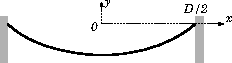
\includegraphics[scale=1.5]{onde1.pdf}
\end{figure}

\begin{itemize}

	\item[$\star$] En appliquant le principe fondamental de la statique sur un élément de corde, déterminer une équation différentielle en $y(x)$, correspondant à la hauteur $y$ de la corde à l'abscisse $x$. On fera apparaître une longueur caractéristique $l_c$, dont on précisera l'expression.
	
	\item[$\star$] Résoudre cette équation différentielle (on pourra résoudre l'équation en utilisant le changement de variable $p(x)=\dif y/\dif x$). Trouver la solution à l'aide des conditions aux limites. 
	
	\item[$\star$] Déterminer la tension $T(x)$ le long de la corde. A quelle endroit est-elle maximale ? Minimale ? Commenter. 
	
	\item[$\star$] Exprimer la longueur $L$ et la \textit{flèche} $h$ (la hauteur entre le point le plus haut et le plus bas) de la chaîne en fonction du paramètre $l_c$. Comment connaître alors la tension dans une chaîne suspendue simplement à partir d'une photographie de celle-ci et de sa masse linéique ?
	
\end{itemize}

\subsubsection*{Cas dynamique}

On considère maintenant que la corde est fortement tendue mais qu'elle n'est plus statique. On cherche à comprendre sa dynamique. On négligera les frottements.

\begin{itemize}

	\item[$\diamond$] Que se passe t-il lorsque la corde devient extrêmement tendue ? Que peut-on négliger par rapport au cas statique ?

	\item[$\diamond$] Déterminer l'équation régissant $y(x,t)$ le long de la corde. Comment s'appelle cette équation ? Quelles sont ses solutions ? Commenter.
	
	\item[$\diamond$] Sachant que la corde est ancrée en $x=0$ et $x=L$, donner l'expression générale de $y(x,t)$ dans le cas de solutions stationnaires. 
	
	\item[$\diamond$] On excite la corde avec une excitation dessinée ci-dessous. Donner l'expression de $y(x,t)$ dans ce cas-là.
	
	\begin{figure}[h!]
	\centering
		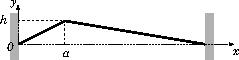
\includegraphics[scale=1.5]{onde2.pdf}
	\end{figure}

	\item[$\diamond$] Si la corde décrite dans l'exercice est celle d'un instrument de musique (violon, guitare, piano...), comment expliquer la différence de timbre entre ces instruments pour une note donnée ?
	
\end{itemize}

\newpage

\section*{Corde pendue verticalement}

On considère une corde attachée au plafond à un point fixe en $z=0$ et laissée verticalement à elle-même dans le vide. Elle n'est soumise qu'à la gravité. On notera $\Psi(z,t)$ l'écart de la corde à la verticale à la hauteur $z$ à l'instant $t$.

\begin{itemize}

	\item[$\ast$] En appliquant le principe fondamental de la dynamique, trouver une équation différentielle en  $\Psi(z,t)$.

\end{itemize}

On cherche des solutions sous la forme $\Psi(z,t)=\alpha(z)\cos(\omega t)+\beta(z)\sin(\omega t)$. 

\begin{itemize}
	
		\item[$\ast$] Comment s'appellent ce type de solutions ? Déterminer l'équation différentielle vérifiée par $\alpha$ et $\beta$.
		
		\item[$\ast$] En posant $Z=\frac{z\omega^2}{g}$, trouver un nouveau système d'équation différentielle en $A(Z)=\alpha(z)/\alpha(0)$. 
		
		\item[$\ast$] On cherche la solution sous la forme d'une série entière $A(Z)=\sum_k A_k Z^K$. Déterminer les coefficients $K$. 
		
		\item[$\ast$] Comment pourrait-on trouver une relation de dispersion $\omega(k)$ ?
		
\end{itemize}

\end{document}
